\documentclass[12pt,a4paper]{article}
\usepackage[margin=1.5cm]{geometry}
\usepackage[T1]{fontenc}
\usepackage[utf8]{inputenc}
\usepackage{lmodern}
\usepackage{booktabs}
\usepackage{tabularx}
\usepackage{array}
\usepackage{enumitem}
\usepackage{xcolor}
\usepackage{hyperref}
\usepackage{microtype}
\usepackage{tikz}
\usetikzlibrary{shapes.geometric, arrows.meta, positioning, calc, fit, backgrounds}

\definecolor{brand}{HTML}{176B52}
\definecolor{brandlight}{HTML}{E8F4F0}
\definecolor{branddark}{HTML}{0E4D3B}
\definecolor{muted}{HTML}{5F716B}
\definecolor{warningbg}{HTML}{FFFBEB}
\definecolor{alertred}{HTML}{B91C1C}

\hypersetup{colorlinks=true,linkcolor=brand,urlcolor=brand,citecolor=brand}
\setlength{\parindent}{0pt}
\setlength{\parskip}{0.55em}

\tikzset{
  flowbox/.style = {rectangle, rounded corners=3pt, draw=brand, fill=brandlight, minimum width=2.6cm, minimum height=0.9cm, text centered, text width=2.5cm, font=\footnotesize\bfseries},
  flowproc/.style = {rectangle, rounded corners=2pt, draw=brand!80, fill=white, minimum width=2.5cm, minimum height=0.8cm, text centered, text width=2.4cm, font=\scriptsize},
  flowdec/.style = {diamond, aspect=1.8, draw=brand, fill=warningbg, minimum width=2.2cm, minimum height=0.8cm, text centered, text width=1.9cm, font=\scriptsize\bfseries},
  flowalert/.style = {rectangle, rounded corners=3pt, draw=alertred, fill=alertred!10, minimum width=2.5cm, minimum height=0.8cm, text centered, text width=2.4cm, font=\scriptsize\bfseries},
  flowterminal/.style = {rectangle, rounded corners=8pt, draw=branddark, fill=branddark, text=white, minimum width=2.4cm, minimum height=0.8cm, text centered, text width=2.3cm, font=\scriptsize\bfseries},
  flowarrow/.style = {thick, -{Stealth[length=2.2mm]}, draw=brand},
  backarrow/.style = {thick, dashed, -{Stealth[length=2.2mm]}, draw=muted},
  alertarrow/.style = {thick, -{Stealth[length=2.2mm]}, draw=alertred}
}

\title{\textbf{Design Concepts and User Story Specification}\\[0.4em]
  \large COMP2300 Deliverable 2 Companion Technical Document\\
  \normalsize Architectural Flowcharts, Decision Matrices, and MoSCoW Story Register}
\author{Arnav Mishra \and Keshav Singhal \and Hiranya Makkar\\[0.4em]
  \small University of Southampton}
\date{November 2026}

\begin{document}
\maketitle

\section{Introduction}
This document provides the detailed engineering specification for the design concepts and user stories formulated for Deliverable 2 (D2) of the COMP2300 project. It details the ideation funnel, formalizes the interaction flowcharts for all three candidate concepts, provides the full Multi-Criteria Decision Matrix, and documents the prioritized user stories with observable acceptance criteria.

\section{Ideation Funnel and Concept Synthesis}

\begin{figure}[ht]
\centering
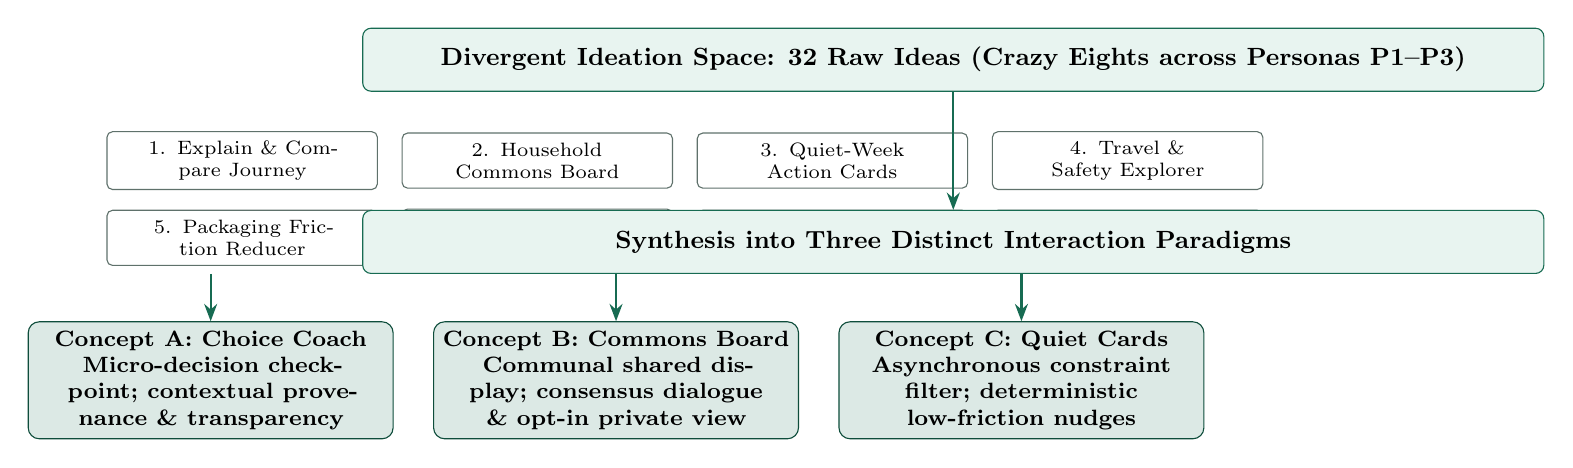
\begin{tikzpicture}[
  node distance=0.55cm and 0.6cm,
  header/.style={rectangle, rounded corners=3pt, draw=brand, fill=brandlight, minimum width=15cm, minimum height=0.8cm, text centered, font=\small\bfseries},
  rfbox/.style={rectangle, rounded corners=2pt, draw=muted, fill=white, minimum width=3.4cm, minimum height=0.7cm, text centered, text width=3.2cm, font=\scriptsize},
  concept/.style={rectangle, rounded corners=4pt, draw=branddark, fill=brand!15, minimum width=4.6cm, minimum height=1.1cm, text centered, text width=4.4cm, font=\footnotesize\bfseries},
  arrow/.style={thick, -{Stealth[length=2.2mm]}, draw=brand}
]
  \node[header] (ideation) {Divergent Ideation Space: 32 Raw Ideas (Crazy Eights across Personas P1--P3)};
  
  \node[rfbox, below left=0.5cm and -0.2cm of ideation] (rf1) {1. Explain \& Compare Journey};
  \node[rfbox, right=0.3cm of rf1] (rf2) {2. Household Commons Board};
  \node[rfbox, right=0.3cm of rf2] (rf3) {3. Quiet-Week Action Cards};
  \node[rfbox, right=0.3cm of rf3] (rf4) {4. Travel \& Safety Explorer};
  
  \node[rfbox, below=0.25cm of rf1] (rf5) {5. Packaging Friction Reducer};
  \node[rfbox, right=0.3cm of rf5] (rf6) {6. Assumptions Audit Explorer};
  \node[rfbox, right=0.3cm of rf6] (rf7) {7. Rota-Aware Scheduler};
  \node[rfbox, right=0.3cm of rf7] (rf8) {8. Offline Conversation Cards};
  
  \node[header, below=1.5cm of ideation] (synth) {Synthesis into Three Distinct Interaction Paradigms};
  
  \node[concept, below left=0.6cm and -0.4cm of synth] (ca) {\textbf{Concept A: Choice Coach}\\Micro-decision checkpoint; contextual provenance \& transparency};
  \node[concept, right=0.5cm of ca] (cb) {\textbf{Concept B: Commons Board}\\Communal shared display; consensus dialogue \& opt-in private view};
  \node[concept, right=0.5cm of cb] (cc) {\textbf{Concept C: Quiet Cards}\\Asynchronous constraint filter; deterministic low-friction nudges};

  \draw[arrow] (ideation) -- (synth);
  \draw[arrow] (synth.south -| ca.north) -- (ca.north);
  \draw[arrow] (synth.south -| cb.north) -- (cb.north);
  \draw[arrow] (synth.south -| cc.north) -- (cc.north);
\end{tikzpicture}
\caption{Divergent-to-Convergent Ideation Funnel: 32 Concepts $\rightarrow$ 8 Families $\rightarrow$ 3 Paradigms}
\end{figure}

\section{Detailed Interaction Flowcharts}

\subsection{Concept A: Contextual Choice Coach (Selected)}
Concept A models carbon footprinting as an inspectable trust checkpoint. Its architectural flowchart details the universal P2 result state, error recovery loops, and constraint branches.

\begin{figure}[ht]
\centering
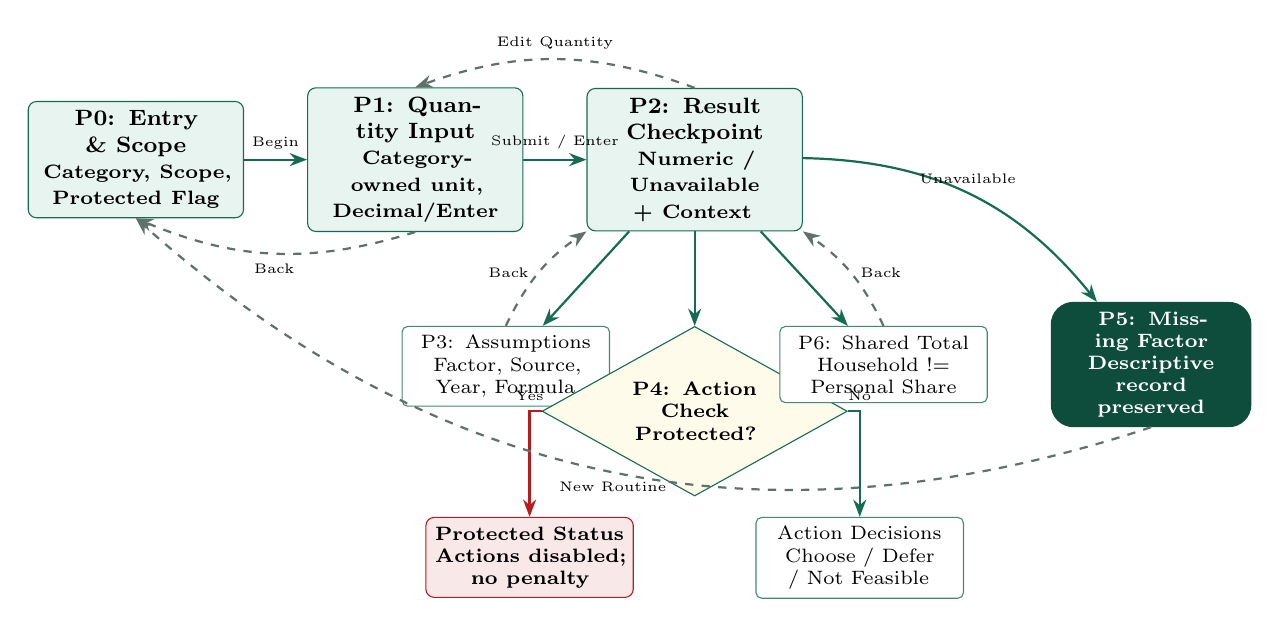
\begin{tikzpicture}[node distance=0.7cm and 0.6cm]
  \node[flowbox] (p0) {P0: Entry \& Scope\\{\scriptsize Category, Scope, Protected Flag}};
  \node[flowbox, right=0.8cm of p0] (p1) {P1: Quantity Input\\{\scriptsize Category-owned unit, Decimal/Enter}};
  \node[flowbox, right=0.8cm of p1] (p2) {P2: Result Checkpoint\\{\scriptsize Numeric / Unavailable + Context}};
  
  \node[flowproc, below left=1.2cm and -0.3cm of p2] (p3) {P3: Assumptions\\{\scriptsize Factor, Source, Year, Formula}};
  \node[flowdec, below=1.2cm of p2] (p4dec) {P4: Action Check\\{\scriptsize Protected?}};
  \node[flowproc, below right=1.2cm and -0.3cm of p2] (p6) {P6: Shared Total\\{\scriptsize Household != Personal Share}};
  
  \node[flowalert, below left=0.8cm and -0.2cm of p4dec] (p4prot) {Protected Status\\{\scriptsize Actions disabled; no penalty}};
  \node[flowproc, below right=0.8cm and -0.2cm of p4dec] (p4act) {Action Decisions\\{\scriptsize Choose / Defer / Not Feasible}};
  \node[flowterminal, right=0.8cm of p6] (p5) {P5: Missing Factor\\{\scriptsize Descriptive record preserved}};

  \draw[flowarrow] (p0) -- node[above, font=\tiny] {Begin} (p1);
  \draw[flowarrow] (p1) -- node[above, font=\tiny] {Submit / Enter} (p2);
  \draw[backarrow] (p1.south) to[bend left=20] node[below, font=\tiny] {Back} (p0.south);
  \draw[backarrow] (p2.north) to[bend right=20] node[above, font=\tiny] {Edit Quantity} (p1.north);
  
  \draw[flowarrow] (p2) -- (p3);
  \draw[flowarrow] (p2) -- (p4dec);
  \draw[flowarrow] (p2) -- (p6);
  \draw[flowarrow] (p2) to[bend left=25] node[above, font=\tiny] {Unavailable} (p5);
  
  \draw[alertarrow] (p4dec) -| node[above, font=\tiny] {Yes} (p4prot);
  \draw[flowarrow] (p4dec) -| node[above, font=\tiny] {No} (p4act);
  
  \draw[backarrow] (p3.north) to[bend left=15] node[left, font=\tiny] {Back} (p2.south west);
  \draw[backarrow] (p6.north) to[bend right=15] node[right, font=\tiny] {Back} (p2.south east);
  \draw[backarrow] (p5.south) to[bend left=30] node[below, font=\tiny] {New Routine} (p0.south);
\end{tikzpicture}
\caption{Detailed Flowchart of Concept A (Footprint Lens Contextual Choice Coach)}
\end{figure}

\subsection{Concept B: Household Commons Board (Communal Coordination)}
Concept B centers on the collective living space. It aggregates communal bills into shared resource cards and facilitates household dialogue without individual policing.

\begin{figure}[ht]
\centering
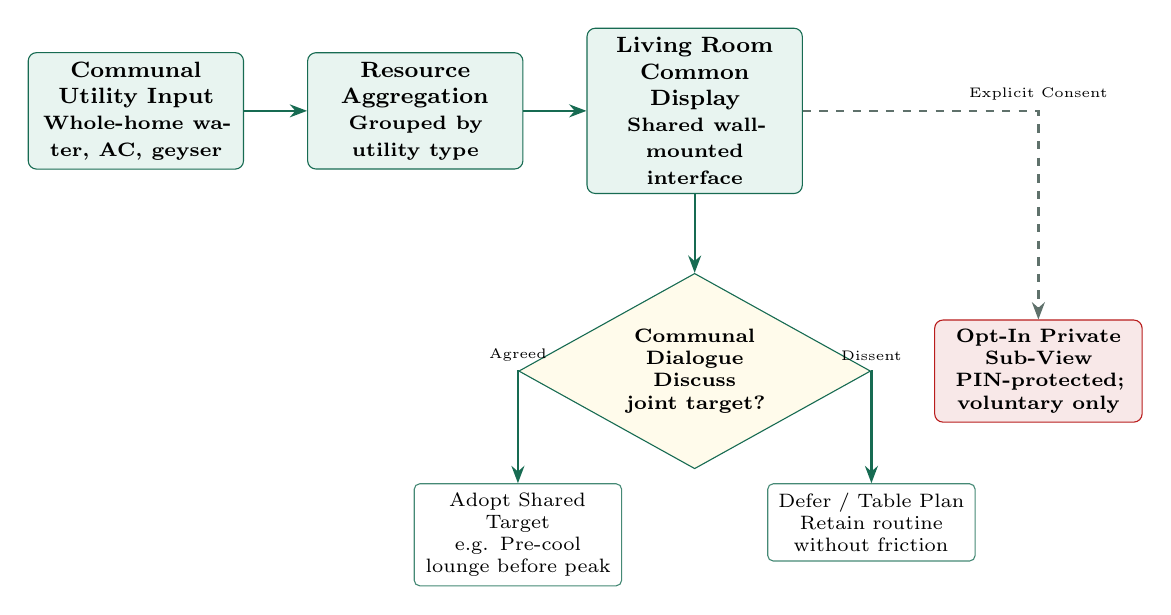
\begin{tikzpicture}[node distance=0.7cm and 0.8cm]
  \node[flowbox] (meters) {Communal Utility Input\\{\scriptsize Whole-home water, AC, geyser}};
  \node[flowbox, right=0.8cm of meters] (agg) {Resource Aggregation\\{\scriptsize Grouped by utility type}};
  \node[flowbox, right=0.8cm of agg] (display) {Living Room Common Display\\{\scriptsize Shared wall-mounted interface}};
  
  \node[flowdec, below=1.0cm of display] (dialogue) {Communal Dialogue\\{\scriptsize Discuss joint target?}};
  \node[flowproc, below left=0.8cm and -0.2cm of dialogue] (target) {Adopt Shared Target\\{\scriptsize e.g. Pre-cool lounge before peak}};
  \node[flowproc, below right=0.8cm and -0.2cm of dialogue] (tabled) {Defer / Table Plan\\{\scriptsize Retain routine without friction}};
  
  \node[flowalert, right=0.8cm of dialogue] (optin) {Opt-In Private Sub-View\\{\scriptsize PIN-protected; voluntary only}};

  \draw[flowarrow] (meters) -- (agg);
  \draw[flowarrow] (agg) -- (display);
  \draw[flowarrow] (display) -- (dialogue);
  \draw[flowarrow] (dialogue) -| node[above, font=\tiny] {Agreed} (target);
  \draw[flowarrow] (dialogue) -| node[above, font=\tiny] {Dissent} (tabled);
  \draw[backarrow] (display) -| node[above, font=\tiny] {Explicit Consent} (optin);
\end{tikzpicture}
\caption{Detailed Flowchart of Concept B (Household Commons Board)}
\end{figure}

\subsection{Concept C: Quiet-Week Action Cards (Asynchronous Nudges)}
Concept C addresses cognitive overload by replacing daily logging with deterministic weekly recommendation cards tailored to external constraints.

\begin{figure}[ht]
\centering
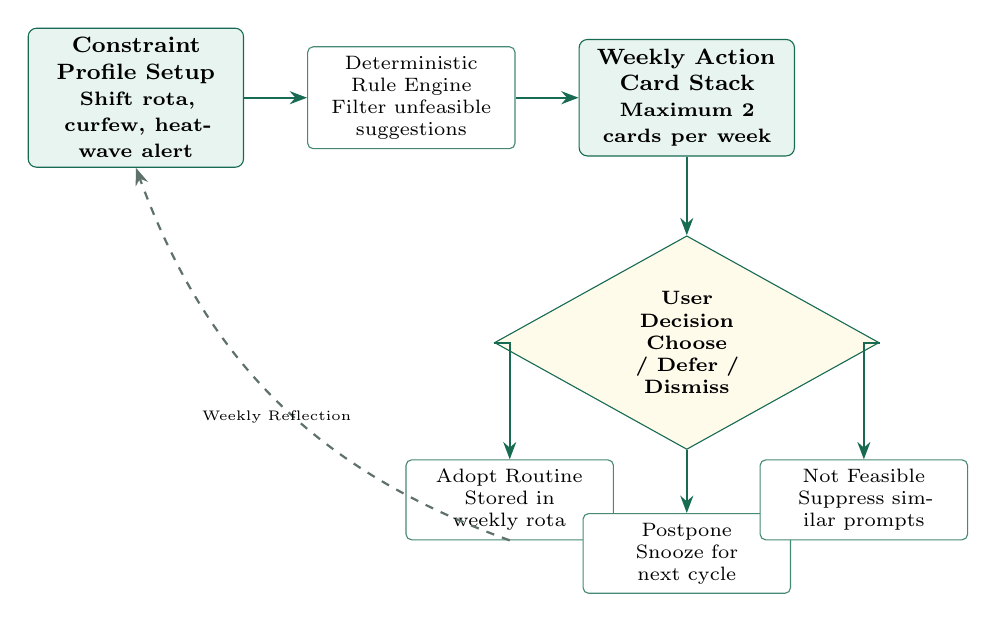
\begin{tikzpicture}[node distance=0.7cm and 0.8cm]
  \node[flowbox] (filter) {Constraint Profile Setup\\{\scriptsize Shift rota, curfew, heatwave alert}};
  \node[flowproc, right=0.8cm of filter] (engine) {Deterministic Rule Engine\\{\scriptsize Filter unfeasible suggestions}};
  \node[flowbox, right=0.8cm of engine] (cards) {Weekly Action Card Stack\\{\scriptsize Maximum 2 cards per week}};
  
  \node[flowdec, below=1.0cm of cards] (decision) {User Decision\\{\scriptsize Choose / Defer / Dismiss}};
  \node[flowproc, below left=0.8cm and -0.3cm of decision] (accept) {Adopt Routine\\{\scriptsize Stored in weekly rota}};
  \node[flowproc, below=0.8cm of decision] (defer) {Postpone\\{\scriptsize Snooze for next cycle}};
  \node[flowproc, below right=0.8cm and -0.3cm of decision] (dismiss) {Not Feasible\\{\scriptsize Suppress similar prompts}};

  \draw[flowarrow] (filter) -- (engine);
  \draw[flowarrow] (engine) -- (cards);
  \draw[flowarrow] (cards) -- (decision);
  \draw[flowarrow] (decision) -| (accept);
  \draw[flowarrow] (decision) -- (defer);
  \draw[flowarrow] (decision) -| (dismiss);
  \draw[backarrow] (accept.south) to[bend left=25] node[below, font=\tiny] {Weekly Reflection} (filter.south);
\end{tikzpicture}
\caption{Detailed Flowchart of Concept C (Quiet-Week Action Cards)}
\end{figure}

\section{Multi-Criteria Decision Analysis (MCDM)}

\begin{table}[ht]
\centering
\small
\caption{Weighted Decision Matrix Justifying Selection of Concept A}
\begin{tabularx}{\textwidth}{@{}lcp{4.2cm}p{4.2cm}p{4.2cm}@{}}
\toprule
\textbf{Criterion} & \textbf{Weight} & \textbf{Concept A: Choice Coach} & \textbf{Concept B: Commons Board} & \textbf{Concept C: Quiet Cards}\\
\midrule
D1 Must Epic Coverage & 25\% & \textbf{5/5:} Fully covers E1--E5 in a single walkthrough. & \textbf{3/5:} Weak on individual action (E3) and brief logging (E5). & \textbf{3/5:} Weak on assumptions (E2) and category coverage (E4).\\
Stakeholder Fit (P1--P3) & 25\% & \textbf{4.5/5:} Balances student flats, shift work, and family budgeting. & \textbf{4/5:} Strong for families (P3), poor for privacy-conscious students (P1). & \textbf{3.5/5:} Good for shift workers (P2), limited for general home tracking.\\
Technical Feasibility & 20\% & \textbf{5/5:} Deterministic rule engine; zero exotic hardware; JavaFX ready. & \textbf{2.5/5:} Multi-user sync, shared device authentication complex. & \textbf{3.5/5:} Requires notification engine and scheduler state.\\
Scientific Provenance & 15\% & \textbf{5/5:} Dedicated P3 assumptions table; transparent factor metadata. & \textbf{3/5:} Aggregated totals obscure underlying conversion formulas. & \textbf{2.5/5:} Recommendation rules detach action from visible evidence.\\
Risk Profile & 15\% & \textbf{4.5/5:} Low risk; false precision mitigated by explicit disclaimers. & \textbf{2/5:} High privacy/coercion risk in multi-tenant environments. & \textbf{3/5:} Risk of appearing like black-box machine learning.\\
\midrule
\textbf{Weighted Score} & \textbf{100\%} & \textbf{4.65 / 5.00 (Selected)} & \textbf{3.00 / 5.00} & \textbf{3.20 / 5.00}\\
\bottomrule
\end{tabularx}
\end{table}

\section{Comprehensive MoSCoW User Story Register}

\begin{table}[ht]
\centering
\scriptsize
\caption{Complete User Story Register (Must, Should, Could, Won't Have)}
\begin{tabularx}{\textwidth}{@{}p{1.2cm}p{1.2cm}p{1.5cm}Xp{5.0cm}@{}}
\toprule
\textbf{ID / Epic} & \textbf{MoSCoW} & \textbf{Persona} & \textbf{User Story} & \textbf{Verifiable Acceptance Criteria}\\
\midrule
D2-US01 (E1) & \textbf{Must} & P1 (Aanya), P3 (Meera) & As a resident, I want to record an activity with its category, quantity, and scope, so that I can see what is being tracked. & \textbf{Given} an activity category, \textbf{When} a non-negative quantity is entered, \textbf{Then} unit updates automatically and scope is stored without losing form state.\\
D2-US02 (E1) & \textbf{Must} & P1--P3 & As a user, I want numeric estimates paired with familiar context (INR cost or bucket count), so that I can grasp the scale. & \textbf{Given} a valid quantity, \textbf{When} result is rendered, \textbf{Then} display kg CO2 alongside labelled familiar metric; unavailable factors never show 0.\\
D2-US03 (E2) & \textbf{Must} & P2 (Rohan), Evidence-user & As an analytical user, I want to inspect factor, formula, year, and source, so that I can verify assumptions. & \textbf{Given} any result, \textbf{When} user opens P3, \textbf{Then} table shows activity, quantity, factor label, reference year, geography, and source status.\\
D2-US04 (E2) & \textbf{Must} & P1--P3 & As a user, I want invalid inputs rejected with recovery controls, so that errors do not crash the session. & \textbf{Given} negative, blank, or $>10^6$ input, \textbf{When} submitted, \textbf{Then} specific error message displays, focus is set, and previous inputs remain intact.\\
D2-US05 (E3) & \textbf{Must} & P2 (Rohan), Shift-worker & As a shift worker, I want to mark constrained routines as protected, so that I am not blamed for necessary choices. & \textbf{Given} protected flag is checked, \textbf{When} P4 action is viewed, \textbf{Then} action buttons are disabled and explicit non-punitive explanation displays.\\
D2-US06 (E3) & \textbf{Must} & P1, P3 & As a user, I want feasible, non-preachy action options, so that I can act within my realistic boundaries. & \textbf{Given} an unprotected result, \textbf{When} action is opened, \textbf{Then} show one realistic next step with functional Choose, Defer, and Not Feasible buttons.\\
D2-US07 (E4) & \textbf{Must} & P1, P3 & As an urban resident, I want packaging, waste, and repair visible, so that circular habits are acknowledged. & \textbf{Given} packaging or repair category, \textbf{When} previewed, \textbf{Then} system displays descriptive preview (P5) without inventing carbon credits.\\
D2-US08 (E5) & \textbf{Must} & P1--P3 & As a busy user, I want a fast entry path ($\le 60$s, $\le 3$ clicks), so that logging does not waste time. & \textbf{Given} P0, \textbf{When} user loads example or enters quantity and hits Enter, \textbf{Then} result renders in $\le 2$ transitions without mandatory extra forms.\\
D2-US09 (E5) & \textbf{Must} & P1--P3 & As an assistive tech user, I want full keyboard and screen-reader support, so that I can navigate accessibly. & \textbf{Given} keyboard-only navigation, \textbf{When} navigating P0--P6, \textbf{Then} all controls have visible focus rings, status changes are announced via ARIA.\\
\midrule
D2-US10 (E1) & \textbf{Should} & P1, P3 & As a household manager, I want to view a monthly summary of logged routines, so that I can see recurring patterns. & \textbf{Given} multiple logged entries, \textbf{When} summary is opened, \textbf{Then} activities are aggregated by category and unit without cross-unit math errors.\\
D2-US11 (E5) & \textbf{Should} & P2 (Rohan) & As a privacy-conscious user, I want local CSV export of my data, so that my personal routines remain offline. & \textbf{Given} session records, \textbf{When} export is selected, \textbf{Then} standard CSV file downloads locally with zero network transmission.\\
D2-US12 (E2) & \textbf{Should} & P3 (Meera) & As a resident, I want to adjust electricity tariff rates to my state (e.g. Delhi vs Mumbai), for accurate cost comparisons. & \textbf{Given} electricity result, \textbf{When} tariff rate is modified, \textbf{Then} variable cost calculation updates immediately with an illustrative note.\\
\midrule
D2-US13 (E4) & \textbf{Could} & P1 (Aanya) & As a student, I want seasonal monsoon/heatwave routine presets, so that my logging reflects extreme weather. & \textbf{Given} seasonal preset toggle, \textbf{When} activated, \textbf{Then} water/cooling baseline recommendations adjust parameters transparently.\\
D2-US14 (E3) & \textbf{Could} & P3 (Meera) & As a consumer, I want to compare bulk vs single-use delivery packaging, to evaluate e-commerce impact. & \textbf{Given} packaging entry, \textbf{When} compared, \textbf{Then} displays descriptive packaging reduction options without carbon claims.\\
\midrule
D2-US15 (E3) & \textbf{Won't} & P1--P3 & Out of scope: Automated black-box AI predictions that infer lifestyle patterns without user consent. & \textbf{Boundary rationale:} Violates COMP2300 prohibition against speculative machine learning; compromises transparent provenance.\\
D2-US16 (E5) & \textbf{Won't} & P1, P2 & Out of scope: IoT hardware sensors or smart meter API integration. & \textbf{Boundary rationale:} Unfeasible for urban Indian rental flatshares; introduces complex third-party network dependencies.\\
D2-US17 (E3) & \textbf{Won't} & P1--P3 & Out of scope: Social leaderboards or peer-shaming rating mechanisms. & \textbf{Boundary rationale:} Directly contradicts JTBD; promotes guilt and ignores structural socio-economic constraints.\\
\bottomrule
\end{tabularx}
\end{table}

\end{document}

